\begin{figure}[h]
  \begin{center}
    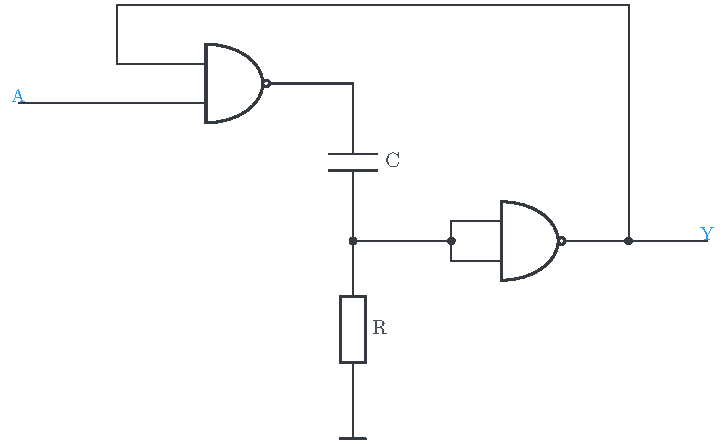
\includegraphics[width=0.618\textwidth]{VBA/3/monoflop}
  \end{center}
  \caption{Monoflopschaltung mit zwei NAND-Gattern}
  \label{fig:monoflop2}
\end{figure}

Die Schaltung aus Abbildung \ref{fig:monoflop2} ist eine Monostabile Kippstufe
mit zwei NAND-Gattern und einer RC-Kombination. Das zweite NAND-Gatter stellt
durch die Verbindung beider Eingangsleitungen einen einfachen Invertierer dar.

Im Ruhezustand (stabiler Zustand) der Schaltung ist Eingang A \HIGH und der
Ausgang des zweiten NAND-Gatters (Y) \HIGH. Durch die Rückkopplung des Ausganges Y wird der Ausgang des ersten
NANDs \LOW und es finden keine Pegeländerungen statt.

Findet nun ein \HIGH \to \LOW Übergang an A statt, wird der Ausgang des ersten
NANDs \HIGH, wodurch der Kondensator C geladen wird. Im Umschaltzeitpunkt des
ersten Gatters liegt dessen volle Ausgangsspannung am Widerstand R an, da der
Kondensator ungeladen ist und über ihn somit keine Spannung abfällt.

Die Spannung über dem Widerstand entspricht der Eingangsspannung des Inverters,
wodurch die Ausgangsspannung zu \LOW wechselt und der Kondensator weiter geladen wird.

Steigt die Spannung über dem Kondensator, so sinkt die Spannung über dem
Widerstand. Ist der Kondensator ausreichend geladen, um die Spannung über dem
Widerstand so verringert zu haben, dass die Eingangsschwelle des Inverters für
die logische Zuordnung (z.B. $2\,\si{\volt}$) unterschritten wird, wechselt der
Ausgang Y auf \HIGH. 

Ändert sich A nun wieder auf \HIGH entlädt sich der Kondensator, da Y=\HIGH und
A=\HIGH und somit der Ausgang des ersten NANDs \LOW ist. Durch den Entladestrom
des Kondensators ist der Spannungsabfall über dem Widerstand negativ in Bezug
auf Masse, weshalb sich der Eingangspegel des Inverters (\LOW) nicht ändert und
Y \HIGH bleibt.

Insgesamt ergibt sich also bei einem Eingangsimpuls ein Ausgangsimpuls, dessen Länge von der
Kondensatorladezeit abhängt.

Für die korrekte Funktion der Schaltung muss darauf geachtet werden, dass die
Länge des Eingangsimpulses deutlich länger ist als die des gewünschten
Ausgangsimpulses, um zu gewährleisten, dass der sich Kondensator ausreichend lädt/entlädt.
Bei zu frühem Wechsel des Eingangssignals auf \LOW bzw. \HIGH kann es daher
vorkommen, dass sich die Ausgangsimpulszeit verändert.

Um die negative Eingangsspannung am Gattereingang zu vermeiden, kann eine Diode
parallel zum Widerstand geschaltet werden. Weiterhin sollte zur Sicherstellung
des Ruhezustandes Eingang A mit einem Pull-Up-Widerstand versehen werden. Die
angepasste Schaltung ist in Abbildung \ref{fig:monoflop3} zu sehen.

\begin{figure}[]
  \begin{center}
    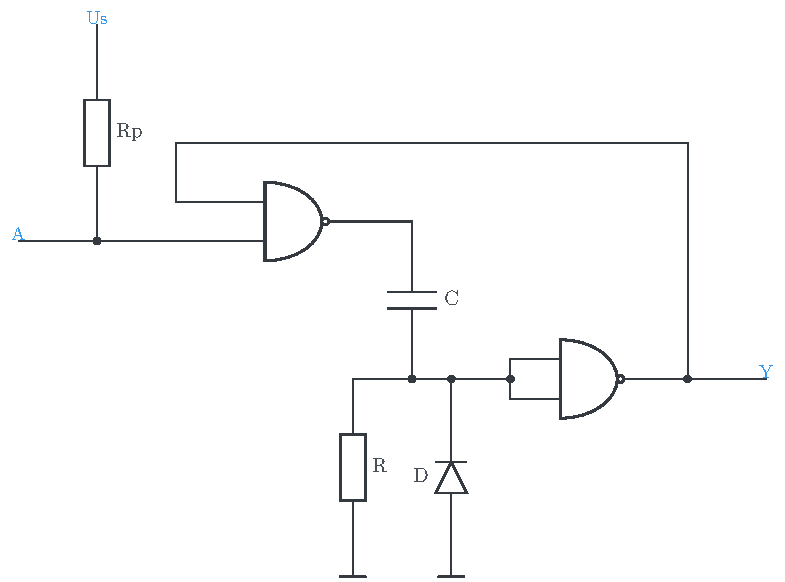
\includegraphics[width=0.618\textwidth]{VBA/3/monoflop2}
  \end{center}
  \caption{Angepasste Monoflopschaltung}
  \label{fig:monoflop3}
\end{figure}
